\documentclass{article}
\usepackage{graphicx}
\usepackage[francais]{babel}
\usepackage[T1]{fontenc}
\usepackage[utf8]{inputenc}
\usepackage{framed}
\PassOptionsToPackage{hyphens}{url}\usepackage{hyperref}

\begin{document}

\title{Rapport sur la Demande de Signature aux Maires de France pour 2017}
\author{Vincent Lamotte}

\maketitle

\section{Introduction}
Ce document présente succinctement les résultats de mon expérience pour récolter les signatures nécessaires à l'élection présidentielle de 2017, en tant que candidat libre. Avec ce status, et aucun financement à ma disposition, ma seule possibilité est de contacter les maires par le biais de courriel. Cette procédure est facilement automatisable à l'aide un script fait maison.

\section{L'envoi des courriels}

\subsection{Les correspondants}

En utilisant les données ouvertes disponibles sur le site internet du gouvernement français, il est possible de récupérer la liste de tous les maires de France, datant du 25 avril 2014 - \url{https://www.data.gouv.fr/fr/datasets/liste-des-maires-au-25-avril-2014/} . Il est possible de récupérer des données sur les maires (35~886 au total), mais pas les adresses électroniques nécessaires.

Avec un second jeu de données, il est possible de récupérer les informations de tous les établissements publics de France, datant du 27 novembre 2015 - \url{https://www.data.gouv.fr/fr/datasets/service-public-fr-annuaire-de-l-administration-base-de-donnees-locales/} . On a alors accès aux mairies ainsi qu'à leur adresse électronique lorsque celle-ci est renseignée.

Une fois ces données croisées, il est possible d'ajouter aux informations des maires l'adresse de leur mairie. En ne ciblant que les maires de France métropolitaine, et en éliminant les mairies sans adresse électronique, on obtient 32~012 correspondants.

\subsection{Le courriel}

Pour assurer que les courriels ne soit pas classés dans la section de spam des mairies, il est nécessaire de configurer le serveur d'envoi avec des options de sécurité. Une fois configuré, le serveur a une note de 8.5/10 sur le service de test de courriel \url{https://www.mail-tester.com/} . Ainsi, on est assuré que les courriels envoyés pourront franchir les filtres de spam.

Le courriel est relativement court, cherchant à mettre en avant l'inspiration des idées défendues. Il contient en pièce jointe une capture du programme à la date de l'envoi. Les courriels sont personalisés avec les noms des maires ainsi que de la commune qu'ils représentent (sections entre crochets dans le courriel).

\begin{framed}
\begin{quotation}
À l’attention de [Nom Maire], maire de la commune de [Commune],\\

Bonjour,

J’ai l’honneur de vous contacter pour vous annoncer ma candidature à l’élection présidentielle de 2017 en tant que candidat libre.

Aujourd’hui, je m’adresse à vous dans l’espoir d’obtenir votre présentation.\\

Les idées de mon programme sont orientées suivant ces grandes lignes :

- Améliorer le système d’élection des représentants des citoyens avec
l’introduction d’un scrutin direct dans les votes de l’Assemblée.

- Diriger les industries vitales pour notre pays vers l’avenir avec la
transition dans les énergies renouvelables, le développement d’une
agriculture raisonnée, et la préservation d’une recherche et d’une
éducation de qualité.

- Favoriser l’égalité dans notre modèle socio-économique en modifiant
les impôts, la fiscalité et les aides sociales.\\

Vous trouverez, en pièce jointe, mon programme complet. Il évolue au quotidien en fonction des propositions citoyennes que je reçois. Vous pouvez trouver la dernière version sur le site web dédié à ma campagne: http://vlamotte.fr/\\

Jeune citoyen de 27 ans, mon programme porte les aspirations et les interrogations d’une jeunesse pragmatique et volontaire qui est désabusée par les partis politiques traditionnels. Nous pensons qu’il est nécessaire de réformer nos institutions pour les rendre plus proches des citoyens. Je défends donc une démocratie efficace, raisonnée et juste. Je suis bien conscient que ma candidature doit vous paraître impossible. Cependant, j’estime que votre soutien apporterait une visibilité certaine à des idées trop souvent mises de côté par les autres candidats.\\

Dans l’attente d’une réponse de votre part, veuillez agréer, [M / Mme / Mlle] la Maire, l'expression de mes respectueuses salutations.\\

Vincent Lamotte
\end{quotation}
\end{framed}

\section{Résultats}
L'envoi des courriels s'est terminé le 20 Juin 2016. Je vous propose les résultats de l'expérience à la date de parution de ce document.

\begin{figure}[h]
    \centering
    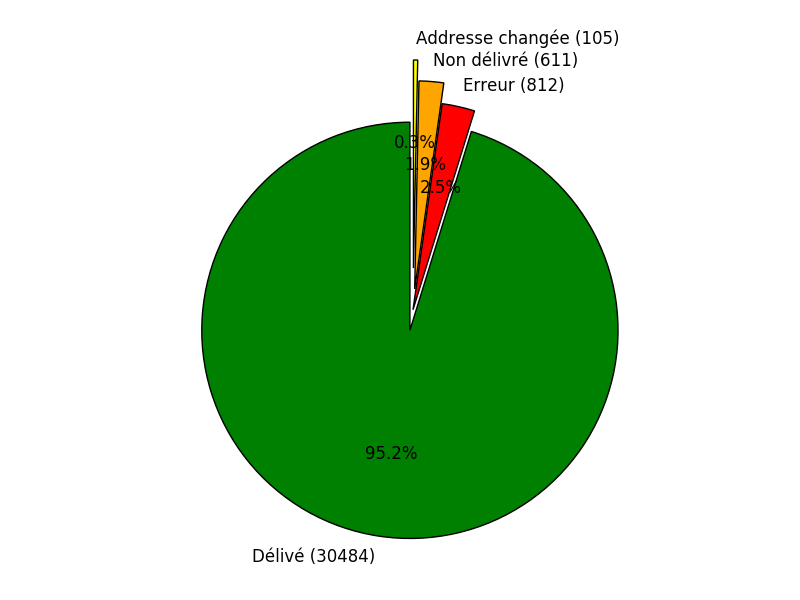
\includegraphics[width=4in]{send.png}
    \caption{Résultat du script d'envoi SMTP}
    \label{send}
\end{figure}

La figure~\ref{send} donne le résultat du script d'envoi SMTP. Sur les 32~012 maires disponibles, on peut catégoriser les envois comme suit:
\begin{itemize}
\item Erreur : Messages non envoyés car le script a rencontré une erreur SMTP. Il serait possible de renvoyer ces messages.
\item Non délivré : Les messages ont été acceptés par le serveur SMTP mais non délivrés à la destination. L'adresse e-mail n'existe sans doute plus.
\item Adresse changée : L'adresse e-mail de la commune a changé, ou le maire n'est plus le même. La réponse est automatique depuis l'ancien mail ou manuel depuis le secrétariat de la commune. Il serait possible de manuellement rectifier ces mails.
\item Delivré : Les messages ont été délivrés sans erreur à l'envoi.
\end{itemize}

Le premier constat au vue de ces résultats est que de nombreuses mairies sont censées avoir reçu le courriel de candidature. Il ne semble pas être possible de chiffrer le taux de blocage par filtre anti-spam. Le nécessaire ayant était fait lors de l'initialisation du serveur d'envoi, cela ne devrait pas être un problème.\\

\begin{figure}[h]
    \centering
    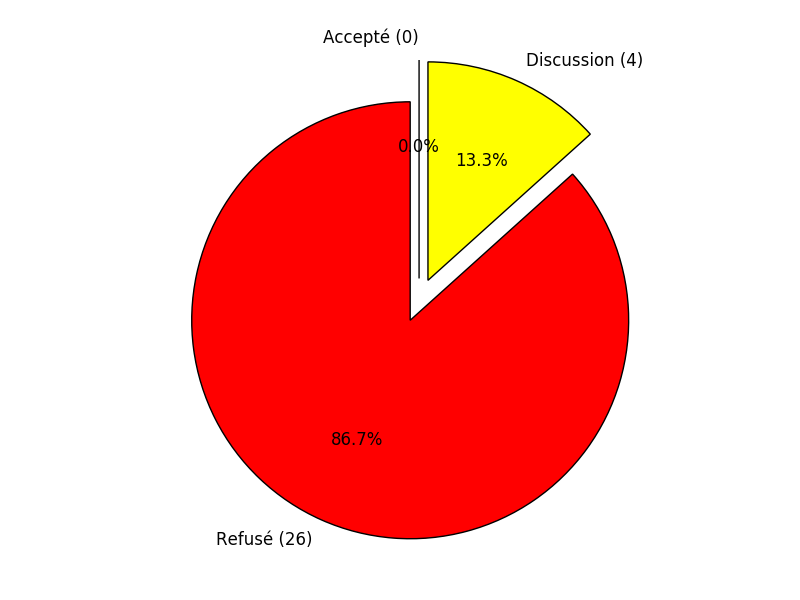
\includegraphics[width=4in]{result.png}
    \caption{Types de Réponses}
    \label{result}
\end{figure}

La figure~\ref{result} indique toutes les réponses reçus des maires. On peut les classer avec les catégories suivantes:
\begin{itemize}
\item Refusé : Les maires ont refusé de donner leur signature pour des raisons variés: signature déjà donnée, blocage contre des idées, parrainage d'aucun candidat.
\item Discussion : Réponse pas claire ou demandant des détails sur le contenu du programme.
\item Accepté : Le maire soutient le programme en envoyant sa signature au conseil constitutionnel.
\end{itemize}

Les réponses sont dans l'ensemble négatives avec parfois la recherche de davantage d'informations qu'il faut gérer individuellement.\\

En complément de la figure~\ref{result}, la figure~\ref{answers} montre le très faible taux de réponse de la part des maires. Il s'agit du nombre de réponses reçues sur l'ensemble des courriels censés être reçus.

\begin{figure}[h]
    \centering
    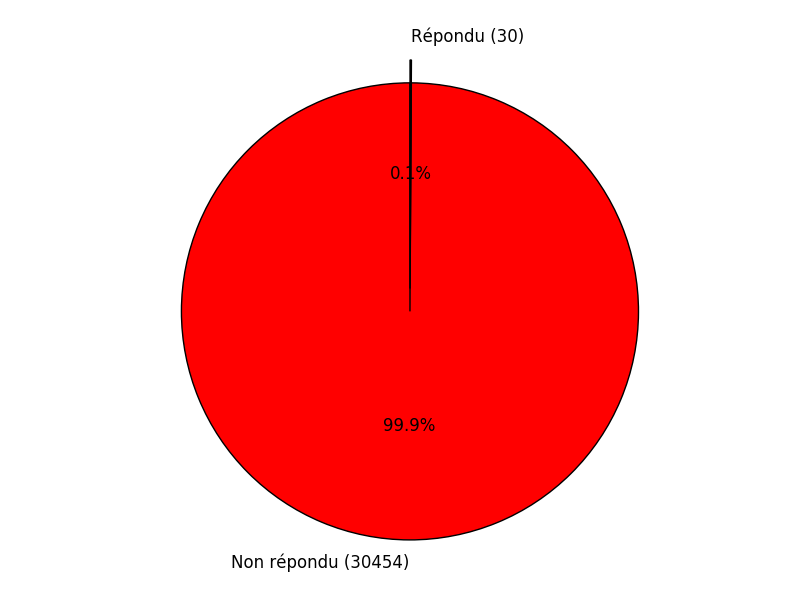
\includegraphics[width=4in]{answers.png}
    \caption{Taux de réponse des Maires}
    \label{answers}
\end{figure}

\section{Conclusion}
Pour conclure, cette expérience met en avant le fait qu'il est très difficile pour un candidat libre d'entrer en contact avec les maires afin d'obtenir leur approbation pour rentrer dans la course politique. Ce système a pour but de filtrer les candidatures farfelues, et il ne fait sans doute que remplir son rôle dans cette expérience.
Cependant, les idées défendues par le programme ne sont pas si absurdes que cela. Pour tenter d'examiner la force de pression de l'opinion publique et des médias, je vais par la suite essayer de transmettre les idées sur les réseaux sociaux pour toucher plus de gens, étant donné que le programme est resté en sous-marin pendant un moment.

\end{document}
